%------------------------------------------------------------
\begin{frame}%{Sharing and disseminating}

\huge{Sharing and disseminating your project}

\end{frame}

%-------------------------------------------
\begin{frame}{Sharing and disseminating}

Goals of this session:

\begin{itemize}
    \item Showcase your work
    \item Add a licence
    \item Create a release
    \item Obtain a DOI for the project
\end{itemize}

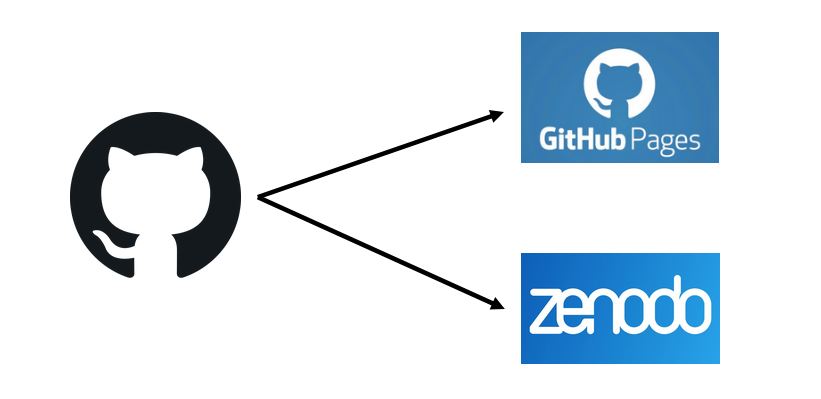
\includegraphics[width=10cm]{08_sharing/images/from_github.png}

\end{frame}

%------------------------------------------------------------
\subsection{Showcase your work}

%------------------------------------------------------------
\begin{frame}{}

\huge{Showcase your work}

\end{frame}

%-------------------------------------------
\begin{frame}{Showcase your work}

\centering
\includegraphics[width=6cm]{08_sharing/images/github_pages.png}

\end{frame}

%-------------------------------------------
\begin{frame}{Showcase your work}

\begin{center}
    
\includegraphics[width=2cm]{08_sharing/images/github_pages.png}
\end{center}

Why ? 

\begin{itemize}
    \item Your project is simpler to share and find
\end{itemize}

Advantages

\begin{itemize}
    \item Free hosting of static websites
    \item Able to convert Markdown into a website
\end{itemize}

Documentation : https://pages.github.com/
\end{frame}

%-------------------------------------------
\begin{frame}{Showcase your work}

In practice

From the main page of your repository, go to :
\begin{itemize}
    \item "Settings" tab
    \item $\,\to\,$ "Options" (left hand side menu)
    \item $\,\to\,$ navigate to the "GitHub Pages" paragraph.
\end{itemize}

\begin{center}
    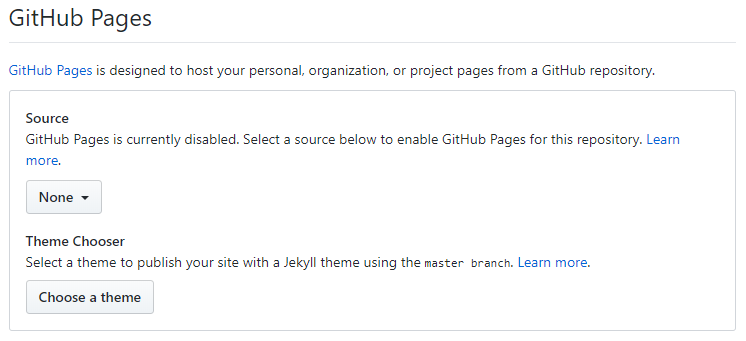
\includegraphics[width=10cm]{08_sharing/images/github_pages_settings.png}
\end{center}

\end{frame}

%-------------------------------------------
\begin{frame}{Showcase your work}

In practice

From the main page of your repository, go to "Settings" $\,\to\,$ "Options" $\,\to\,$ "GitHub Pages".

\begin{enumerate}
    \item Choose the source
\end{enumerate}

\begin{center}
    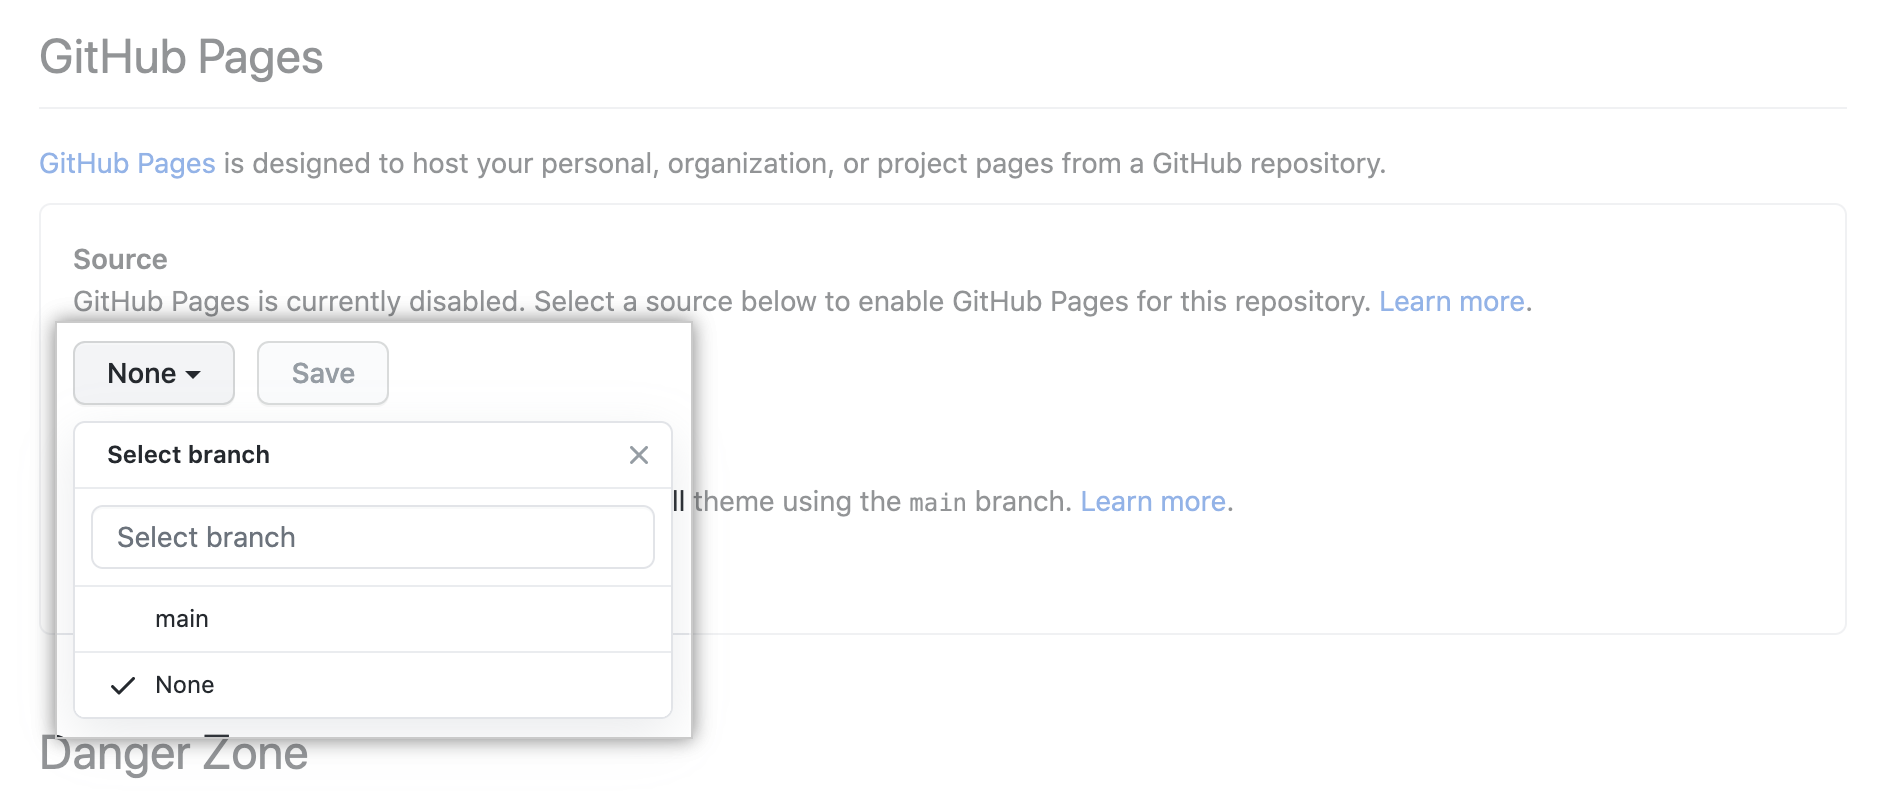
\includegraphics[width=10cm]{08_sharing/images/github_pages_settings_branch.png}
\end{center}

\end{frame}

%-------------------------------------------
\begin{frame}{Showcase your work}

In practice

From the main page of your repository, go to "Settings" $\,\to\,$ "Options" $\,\to\,$ "GitHub Pages".

\begin{enumerate}
    \item Choose the source
\end{enumerate}

\begin{center}
    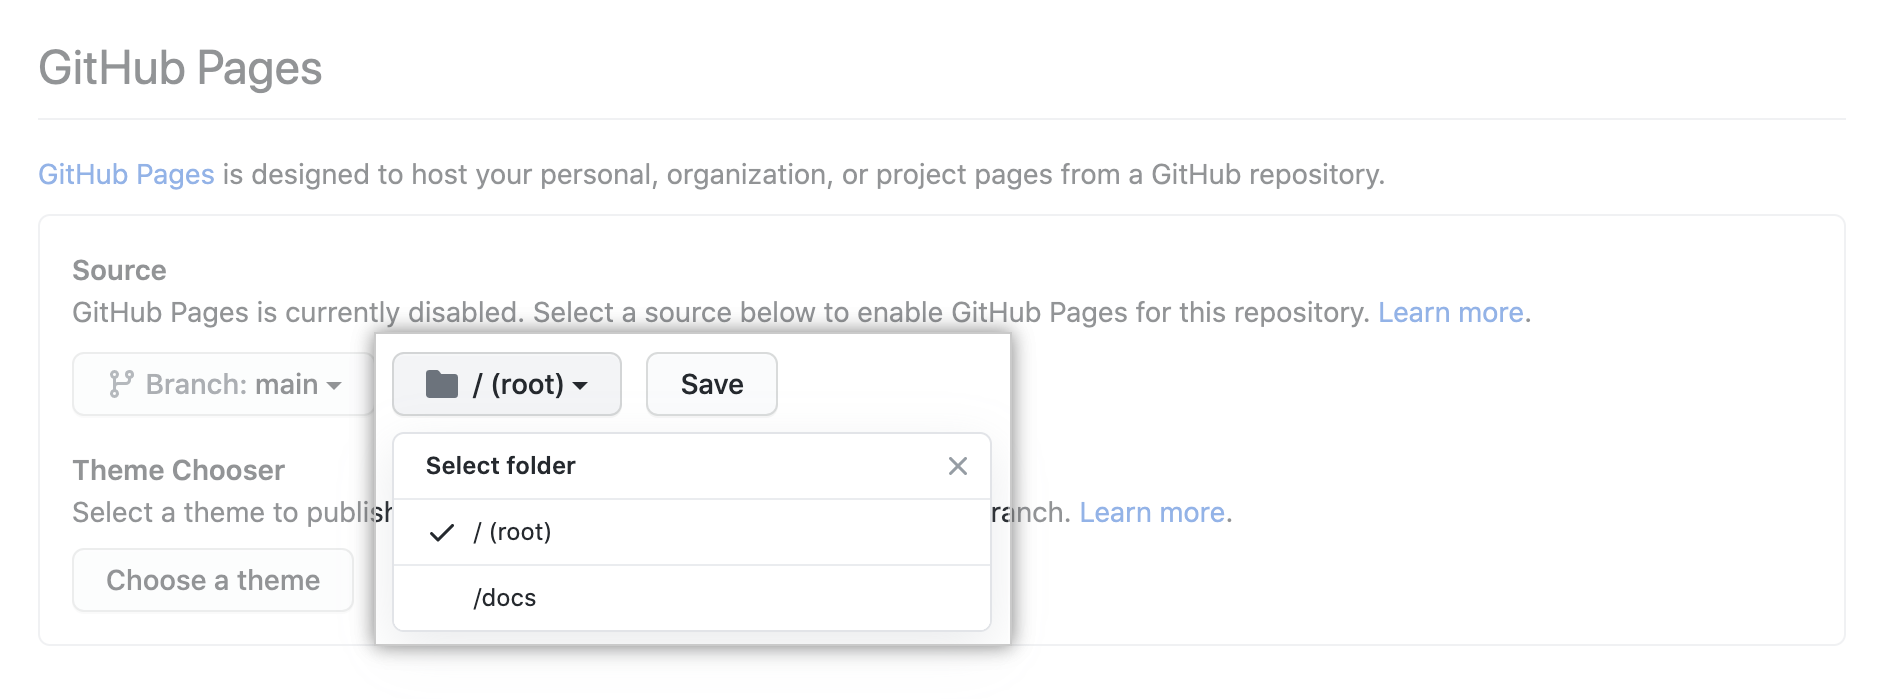
\includegraphics[width=10cm]{08_sharing/images/github_pages_settings_folder.png}
\end{center}

\end{frame}

%-------------------------------------------
\begin{frame}{Showcase your work}

In practice

From the main page of your repository, go to "Settings" $\,\to\,$ "Options" $\,\to\,$ "GitHub Pages".

\begin{enumerate}
    \item Choose the source
\end{enumerate}

\begin{center}
    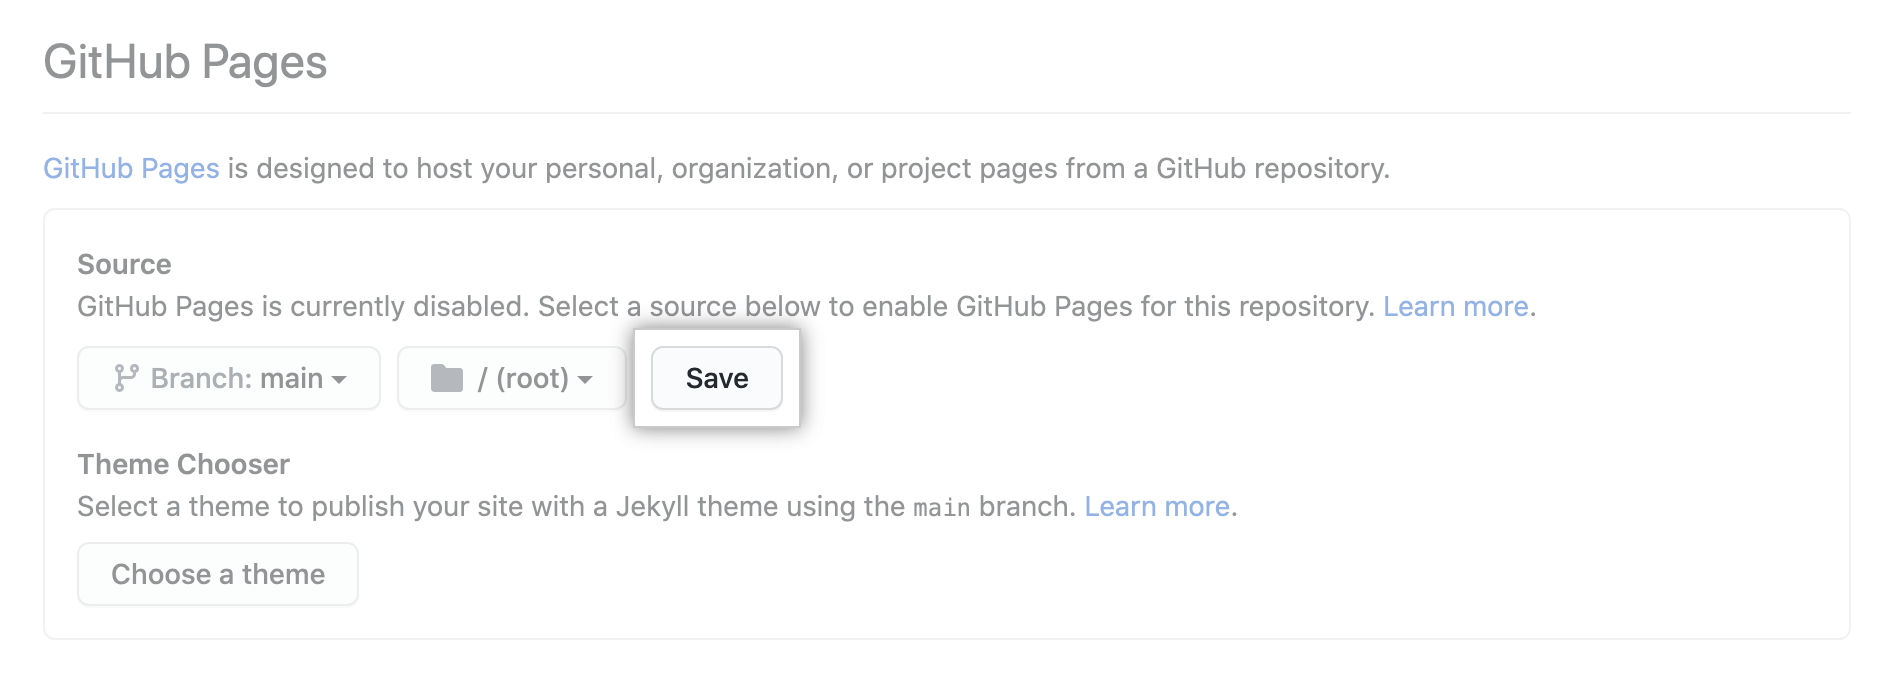
\includegraphics[width=10cm]{08_sharing/images/github_pages_settings_save.png}
\end{center}

\end{frame}

%-------------------------------------------
\begin{frame}{Showcase your work}

In practice

From the main page of your repository, go to "Settings" $\,\to\,$ "Options" $\,\to\,$ "GitHub Pages".

\begin{enumerate}
    \item Choose the source
    \item Choose the theme
\end{enumerate}

\begin{center}
    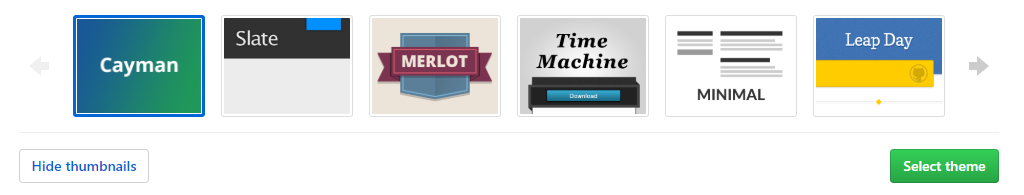
\includegraphics[width=10cm]{08_sharing/images/github_pages_settings_theme.png}
\end{center}

\end{frame}

%-------------------------------------------
\begin{frame}{Showcase your work}

Convert Markdown into HTML !

\begin{center}
    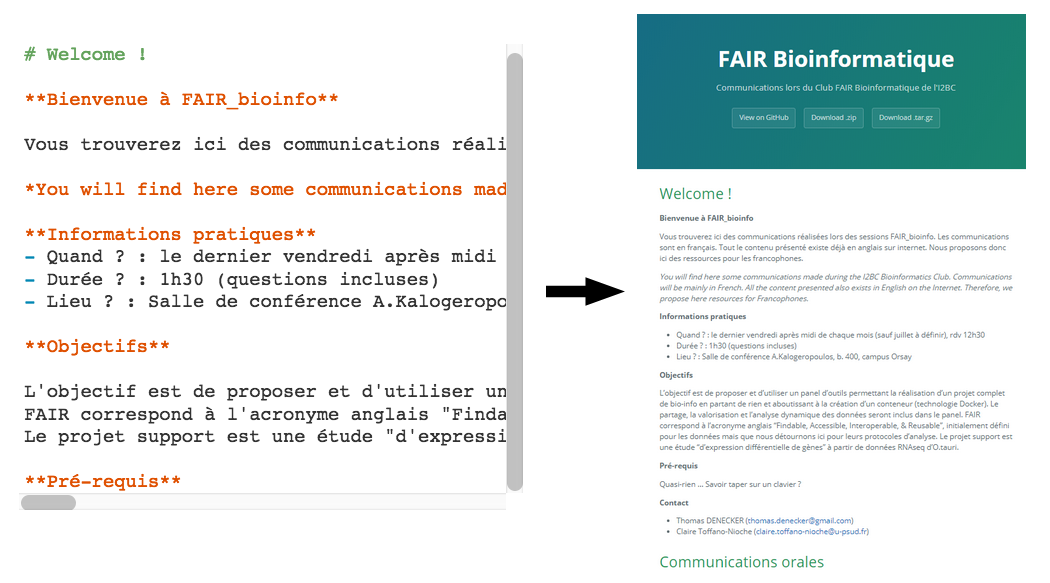
\includegraphics[width=10cm]{08_sharing/images/convert_html.png}
\end{center}

\begin{center}
\url{https://thomasdenecker.github.io/FAIR_Bioinfo}
\end{center}

\end{frame}

%-------------------------------------------
\begin{frame}{Showcase your work}

Also works directly from HTML 

\begin{enumerate}
    \item Create a folder named "docs"
    \begin{itemize}
        \item main file must be named index.html
    \end{itemize}
    \item "Settings" $\,\to\,$ "Options" $\,\to\,$ "GitHub Pages"
\end{enumerate}

\begin{center}
    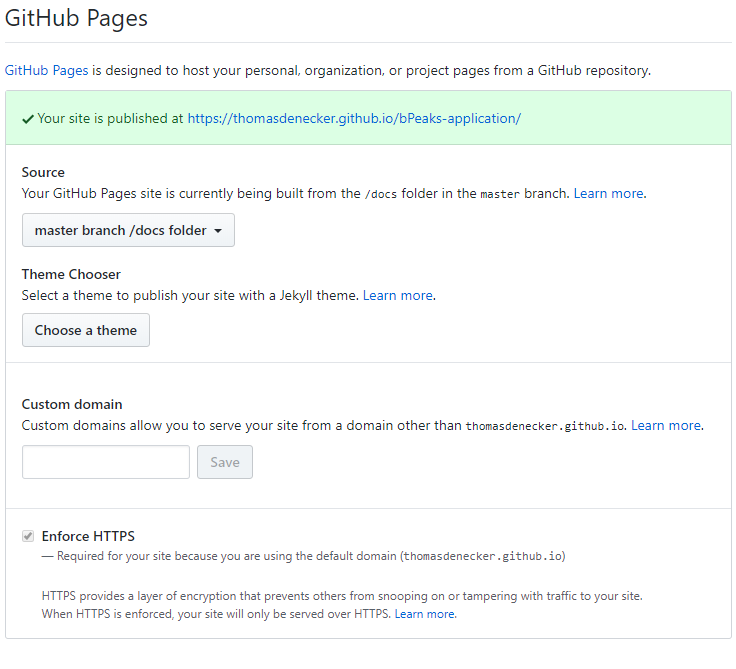
\includegraphics[width=5cm]{08_sharing/images/github_pages_settings_html.png}
\end{center}

\begin{center}
\url{https://thomasdenecker.github.io/bPeaks-application/}
\end{center}

\end{frame}

%-------------------------------------------
\begin{frame}{Showcase your work}

Remember to choose a licence !

This will determine whether anyone can use, modify, and distribute your code / tool / software...

\begin{center}
\url{https://help.github.com/en/articles/licensing-a-repository}
\end{center}

\begin{enumerate}
    \item Create a file named "LICENCE"
    \item GitHub will suggest templates
\end{enumerate}

\begin{center}
    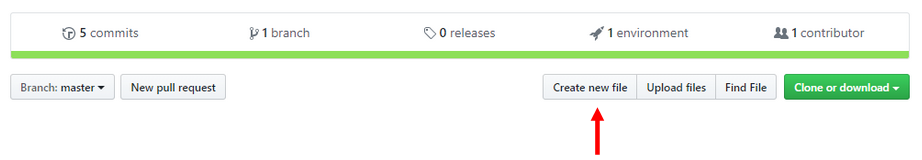
\includegraphics[width=10cm]{08_sharing/images/github_new_file.png}
\end{center}

\end{frame}

%-------------------------------------------
\begin{frame}{Showcase your work}

Remember to choose a licence !

This will determine whether anyone can use, modify, and distribute your code / tool / software...

\begin{center}
\url{https://help.github.com/en/articles/licensing-a-repository}
\end{center}

\begin{enumerate}
    \item Create a file named "LICENCE"
    \item GitHub will suggest templates
\end{enumerate}

\begin{center}
    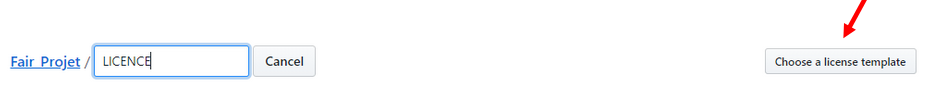
\includegraphics[width=10cm]{08_sharing/images/github_licence.png}
\end{center}

The CeCILL licence (v.2.1) is recommended by the CEA, CNRS and INRIA ("CEA CNRS INRIA Logiciel Libre"). Copy it directly. 
\url{http://cecill.info/licences.fr.html}
\end{frame}

%-------------------------------------------
\begin{frame}{Showcase your work}

GitHub takes care of displaying the information on your repository.

\begin{center}
    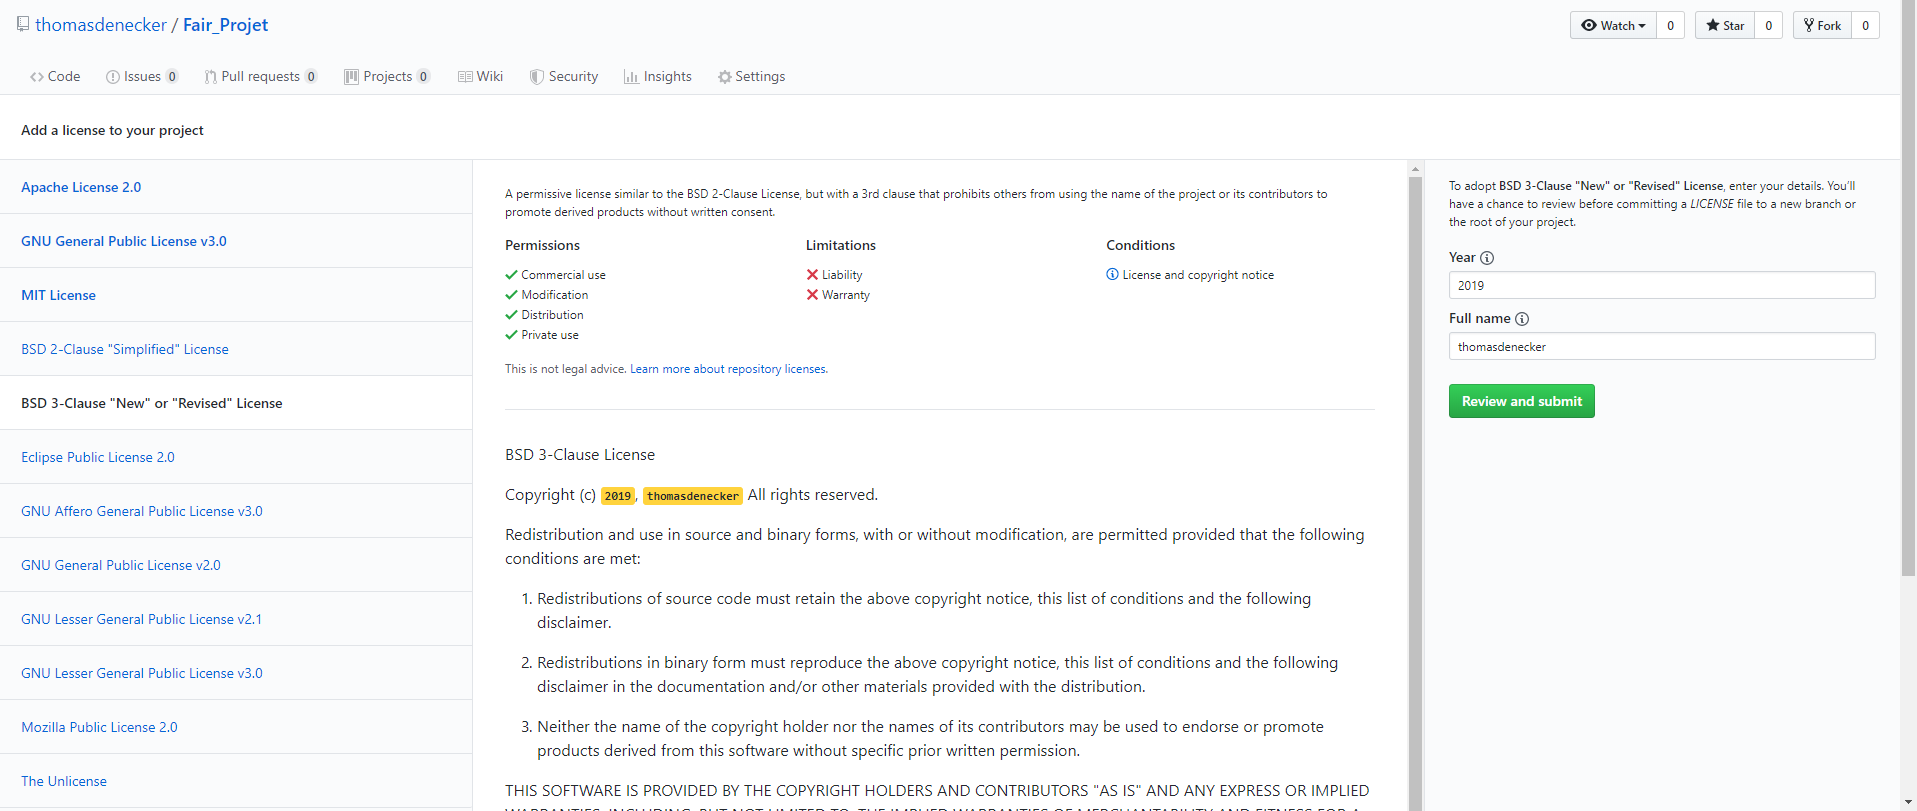
\includegraphics[width=10cm]{08_sharing/images/github_licence_show.png}
\end{center}

\end{frame}

%-------------------------------------------
\begin{frame}{Showcase your work}

Validate and merge with the main branch

\begin{center}
    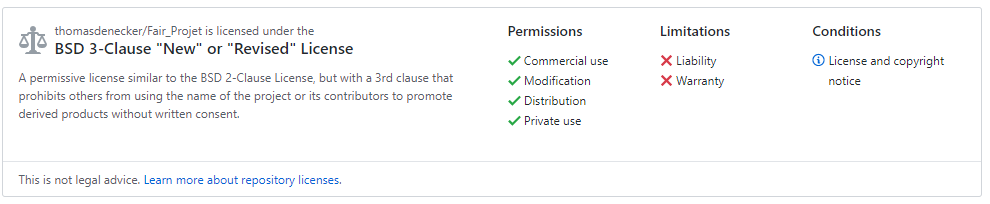
\includegraphics[width=10cm]{08_sharing/images/github_licence_details.png}
\end{center}

\end{frame}

%-------------------------------------------
\begin{frame}{Showcase your work}

Kind reminder: consequence of not choosing a licence.

\begin{center}
    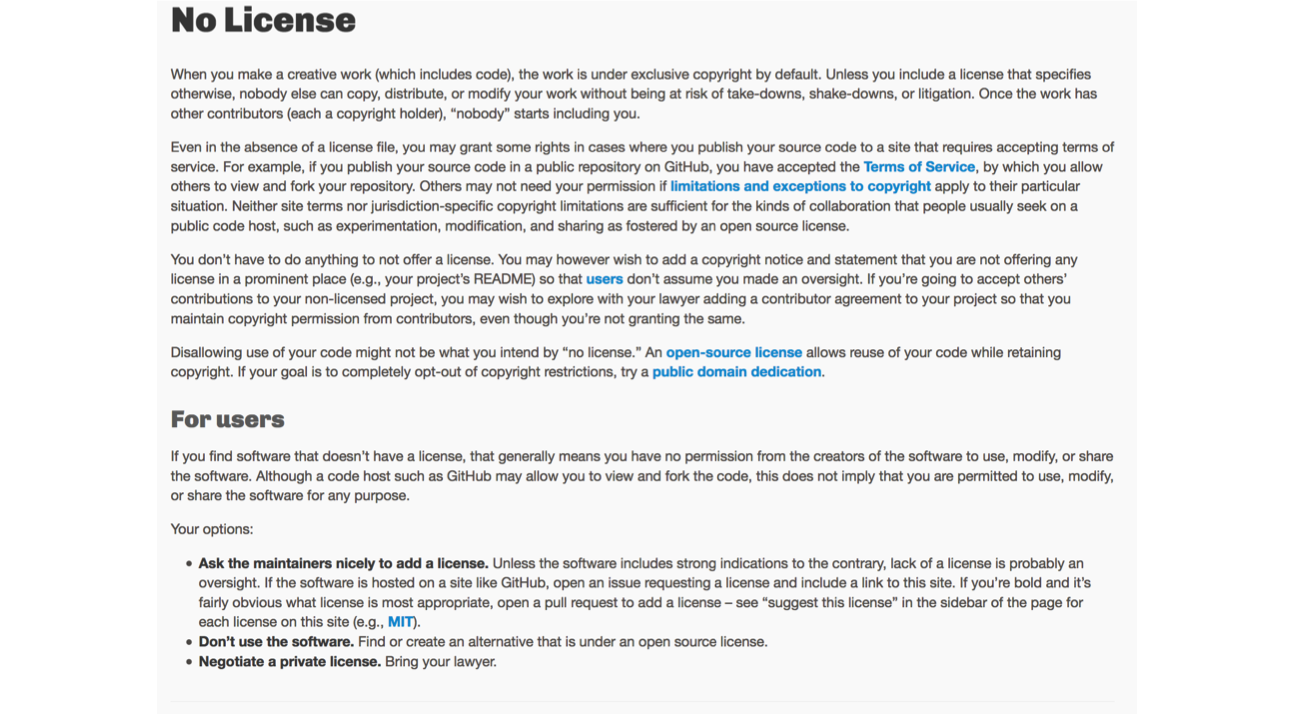
\includegraphics[width=12cm]{08_sharing/images/github_nolicence.png}
\end{center}

\end{frame}

%------------------------------------------------------------
\subsection{Release}

%------------------------------------------------------------
\begin{frame}{}

\huge{Release}

\end{frame}

%-------------------------------------------
\begin{frame}{Release}

Goal : provide users with a version of your code that has been fixed in time and labelled.

All the steps are detailed here:

\begin{itemize}
    \item \url{https://help.github.com/en/articles/creating-releases}
\end{itemize}

\end{frame}

%-------------------------------------------
\begin{frame}{Release}

Make a release

\begin{center}
    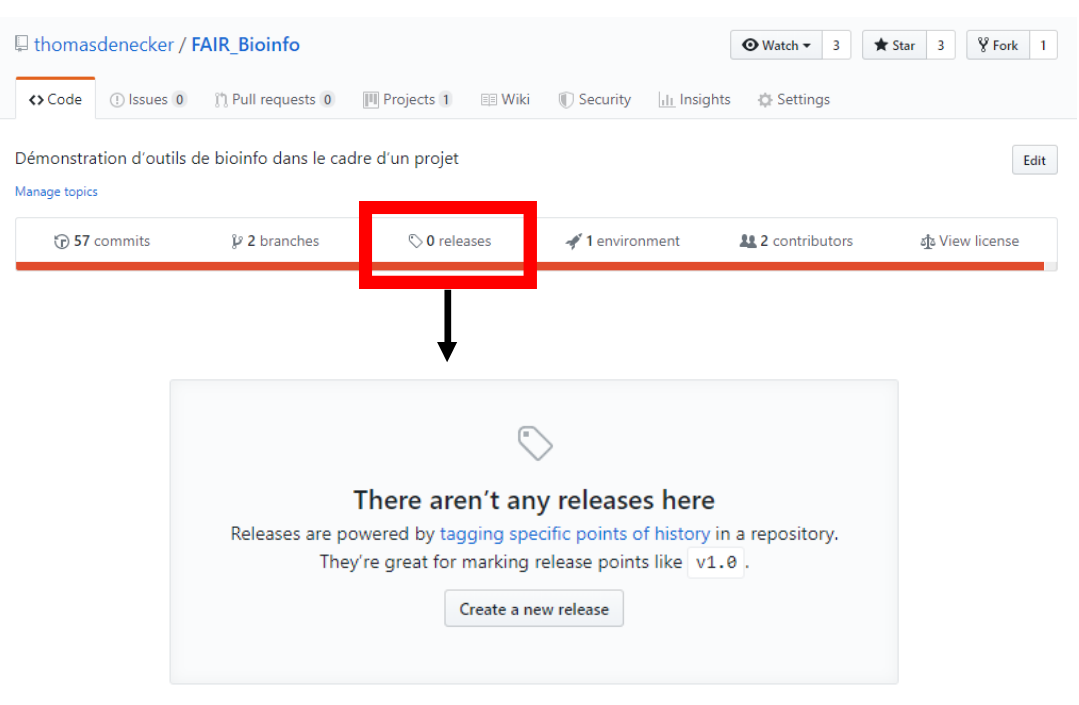
\includegraphics[width=10cm]{08_sharing/images/github_release.png}
\end{center}

\end{frame}

%-------------------------------------------
\begin{frame}{Release}

Make a release

\begin{center}
    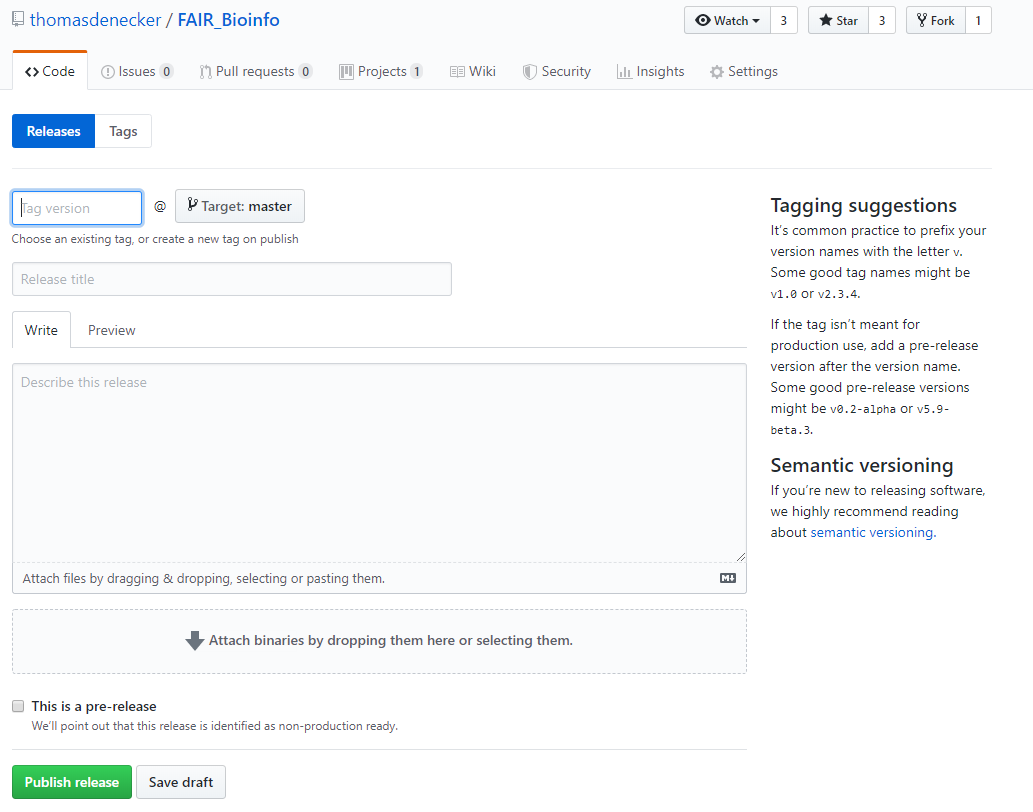
\includegraphics[width=10cm]{08_sharing/images/github_new_release.png}
\end{center}

\end{frame}

%-------------------------------------------
\begin{frame}{Release}

Semantic of a release number

\begin{center}
    \textbf{1.0.0}
    
    MAJOR.MINOR.PATCH
    
\end{center}
\par
\begin{itemize}
    \item MAJOR : changes not backwards-compatible
    \item MINOR : new/modified functionalities, backwards-compatible
    \item PATCH : bug fixes, backwards-compatible
\end{itemize}

More details : \url{https://semver.org/}
\end{frame}

%-------------------------------------------
\begin{frame}{Release}

First release for FAIR\_Bioinfo

\begin{center}
    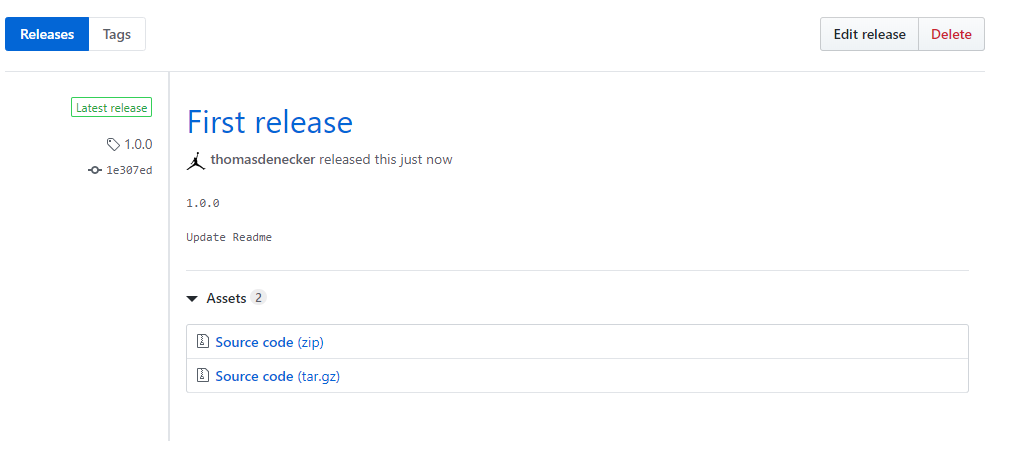
\includegraphics[width=10cm]{08_sharing/images/github_first_release.png}
\end{center}

\end{frame}

%------------------------------------------------------------
\subsection{Obtain a DOI}

%------------------------------------------------------------
\begin{frame}{}

\huge{Obtain a DOI}

\end{frame}


%-------------------------------------------
\begin{frame}{Obtain a DOI}

\begin{center}
    
\includegraphics[width=8cm]{08_sharing/images/zenodo.png}
\end{center}

\end{frame}

%-------------------------------------------
\begin{frame}{Obtain a DOI}

\textbf{D}igital \textbf{O}bject \textbf{I}dentifier

Reference system to cite an object (A GitHub project in our case)

\begin{center}
    
\includegraphics[width=4cm]{08_sharing/images/zenodo.png}
\end{center}

\url{https://guides.github.com/activities/citable-code/}
\end{frame}

%-------------------------------------------
\begin{frame}{Obtain a DOI}

1/ Sign in to Zenodo

\begin{itemize}
    \item With your GitHub account
    \item With your ORCID account (add a "Linked account" to GitHub afterwards)
\end{itemize}

2/ Go to the Settings page $\,\to\,$ GitHub tab

\begin{center}
    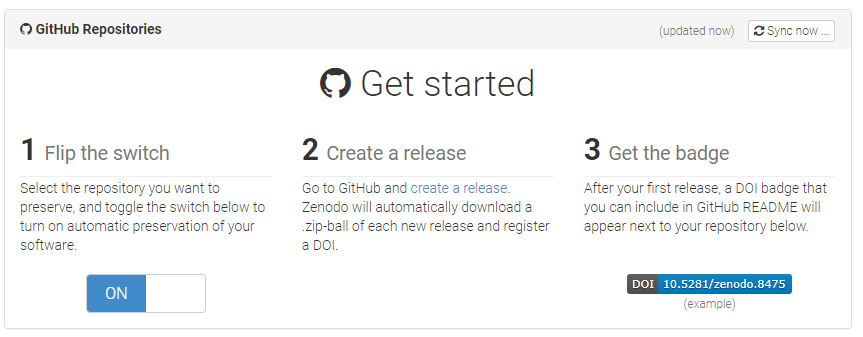
\includegraphics[width=7cm]{08_sharing/images/zenodo_github.png}
\end{center}


\end{frame}

%-------------------------------------------
\begin{frame}{Obtain a DOI}

{\centering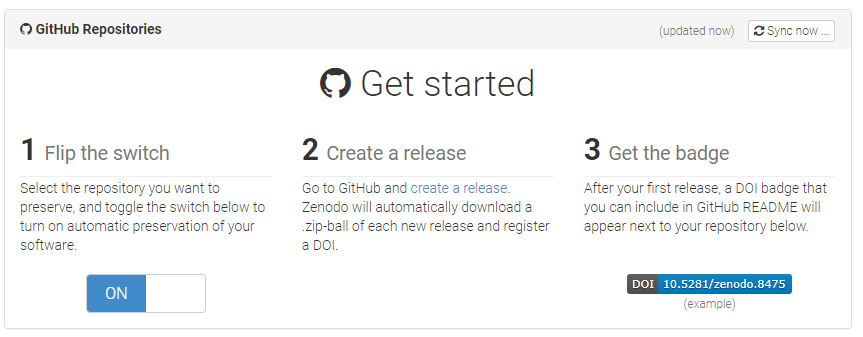
\includegraphics[width=7cm]{08_sharing/images/zenodo_github.png}\par }

3/ In the list below, find the project you want to link to Zenodo. Flip the switch.

\begin{center}
    
\includegraphics[width=10cm]{08_sharing/images/zenodo_link.png}
\end{center}

\end{frame}

%-------------------------------------------
\begin{frame}{Obtain a DOI}

{\centering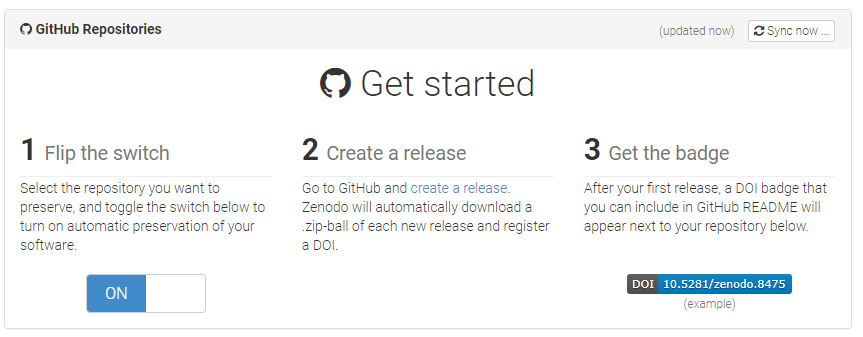
\includegraphics[width=7cm]{08_sharing/images/zenodo_github.png}\par }

4/ On GitHub, in Settings $\,\to\,$ Webhooks, a new line has been created: Zenodo will be notified of any new release created in this project.

\begin{center}
    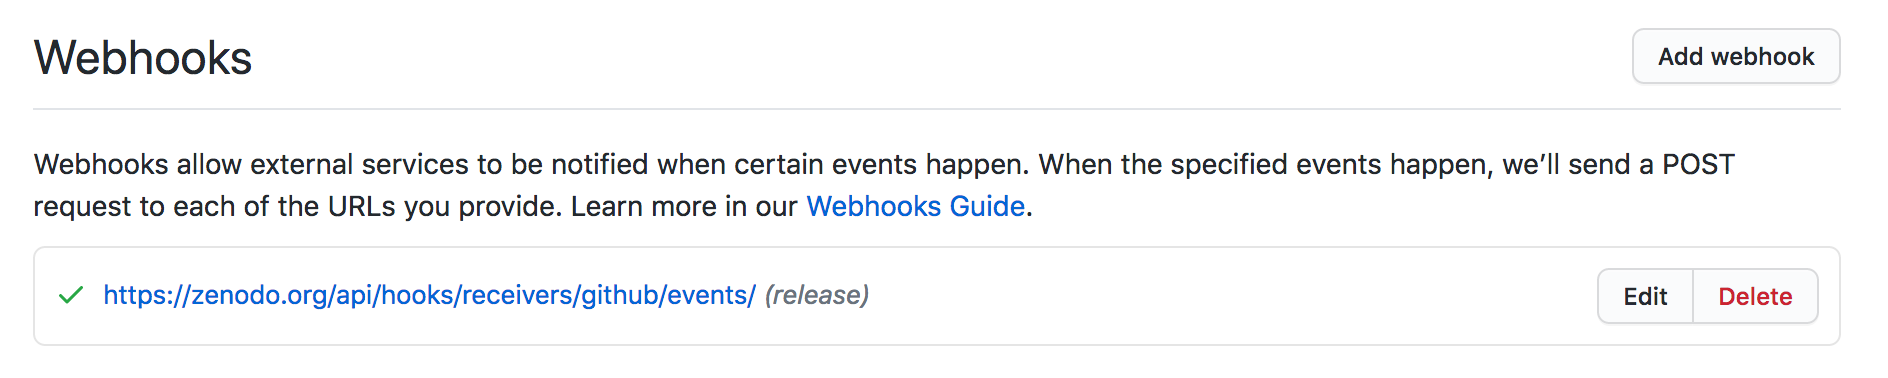
\includegraphics[width=10cm]{08_sharing/images/webhook_zenodo.png}
\end{center}

\end{frame}

%-------------------------------------------
\begin{frame}{Obtain a DOI}

{\centering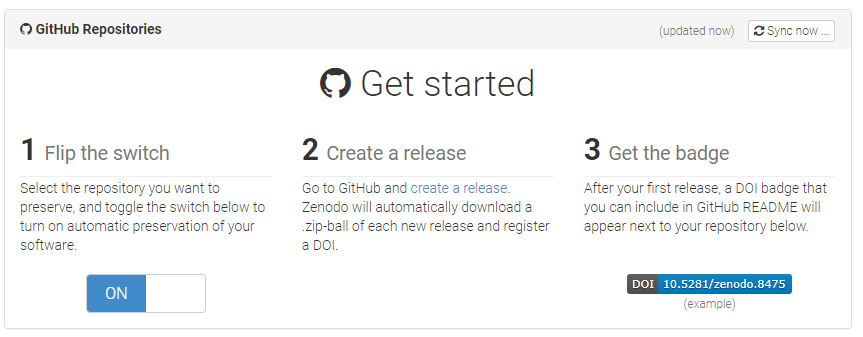
\includegraphics[width=7cm]{08_sharing/images/zenodo_github.png}\par }

5/ Back to Zenodo. After a release, a badge will be available below the project's name, in the category Enabled repositories. 

\begin{center}
    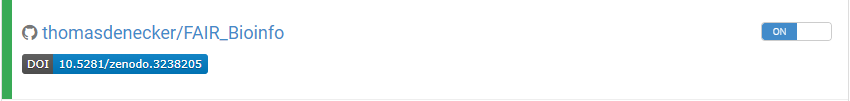
\includegraphics[width=10cm]{08_sharing/images/zenodo_badge.png}
\end{center}

\end{frame}

%-------------------------------------------
\begin{frame}{Obtain a DOI}

\begin{center}
    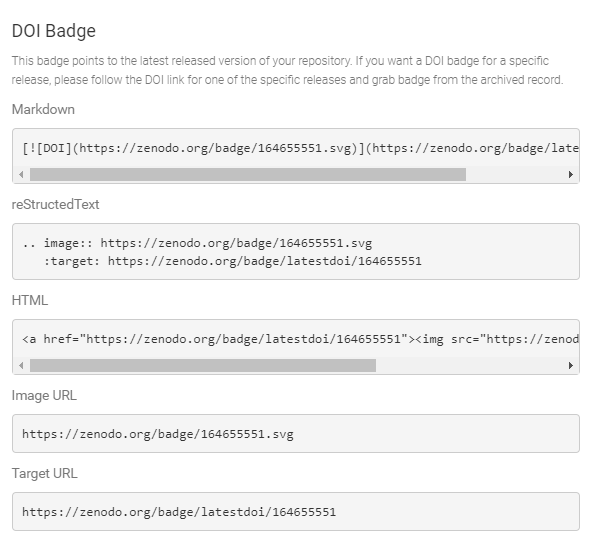
\includegraphics[width=8cm]{08_sharing/images/badge_code.png}
\end{center}

\end{frame}

%-------------------------------------------
\begin{frame}{Obtain a DOI}

{\centering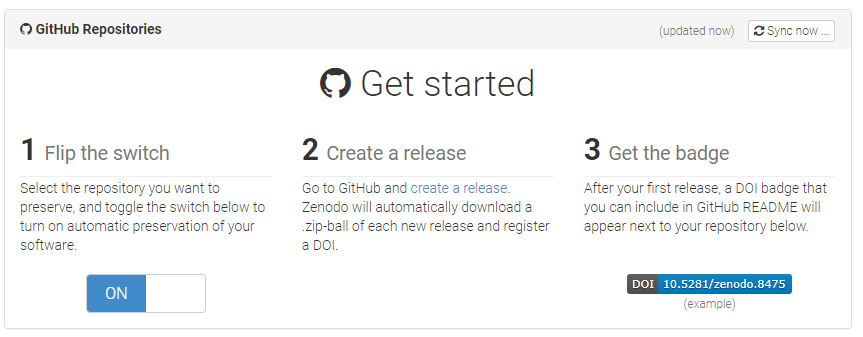
\includegraphics[width=7cm]{08_sharing/images/zenodo_github.png}\par }

6/ Add the code for the badge to the README.

{\centering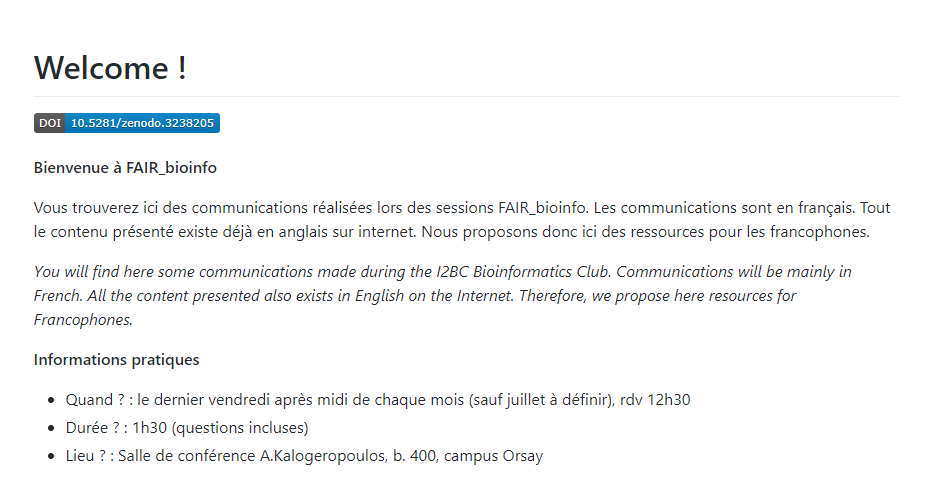
\includegraphics[width=7cm]{08_sharing/images/readme_badge.png}\par }

\end{frame}

%-------------------------------------------
\begin{frame}{GitHub Package Registry}

\begin{columns}

\column{0.5\textwidth}
{\centering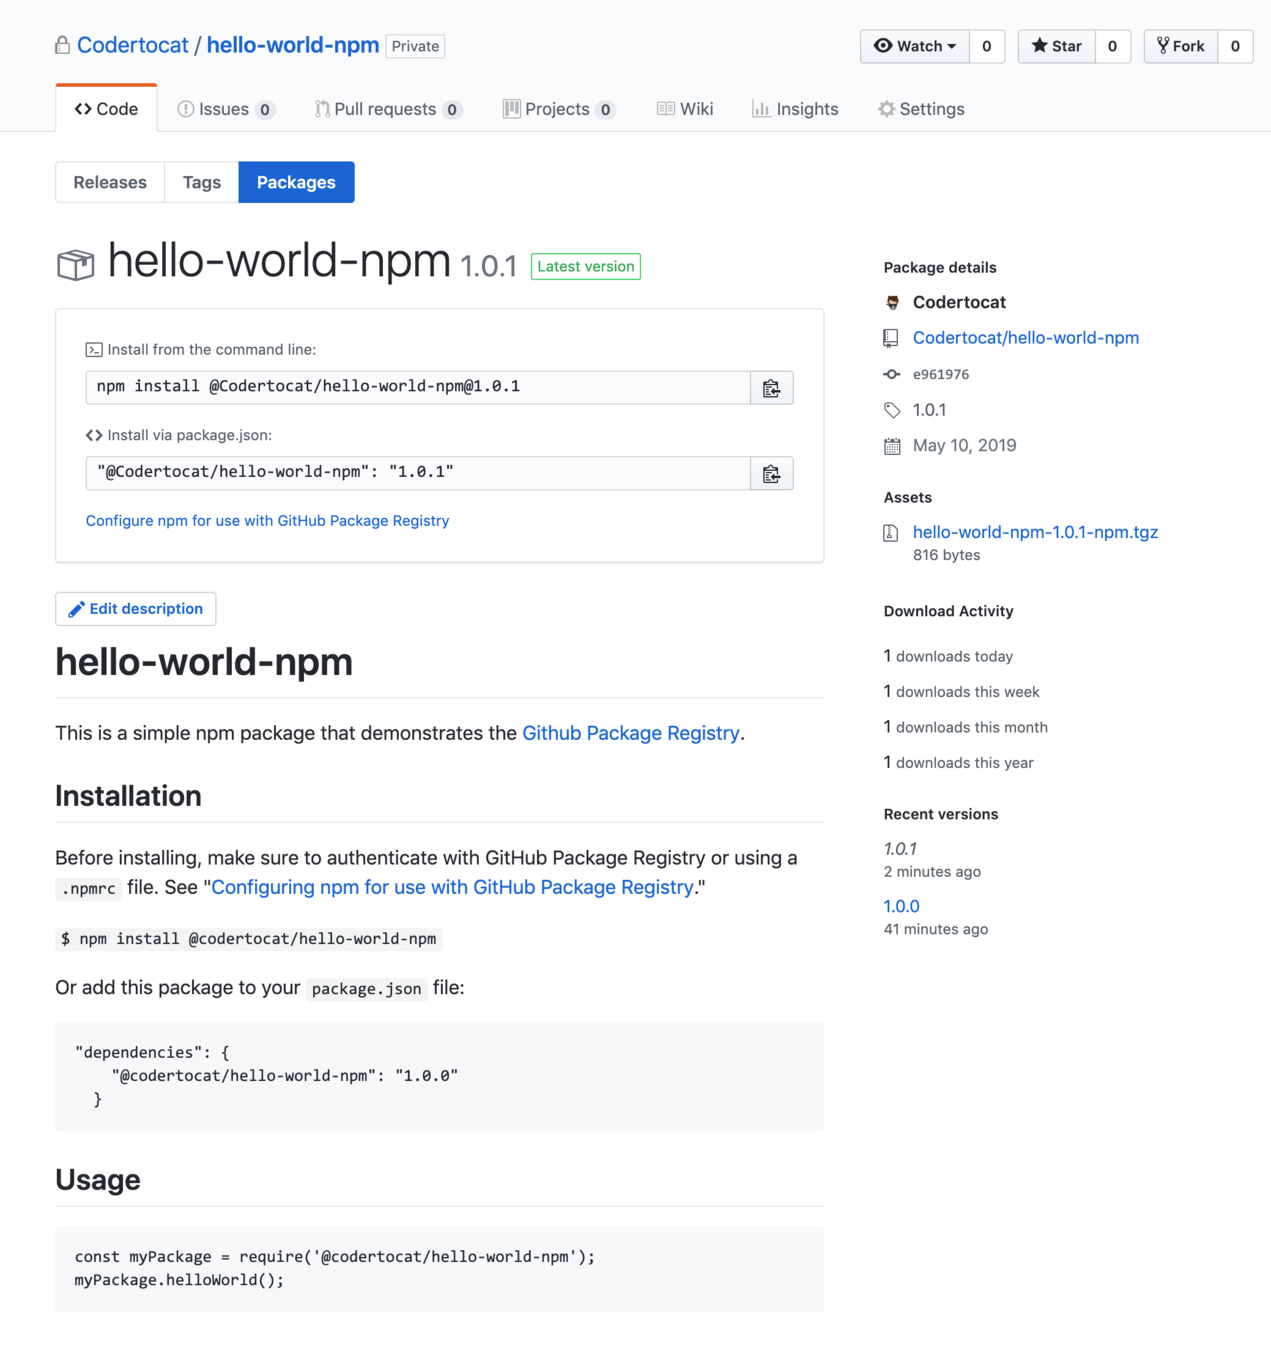
\includegraphics[width=6cm]{08_sharing/images/github_registry.png} \par }

\column{0.5\textwidth}
Packages directly available on GitHub.


\url{https://help.github.com/en/articles/about-github-package-registry}


\url{https://github.com/features/package-registry}

\end{columns}

\end{frame}



